\documentclass[11pt,oneside]{article}



\usepackage[T1]{fontenc}
\usepackage[utf8]{inputenc}
%\usepackage[latin1]{inputenc}
\DeclareUnicodeCharacter{00A0}{ }
% \usepackage{lmodern}
%\usepackage[adobe-utopia,uppercase=upright,greeklowercase=upright]{mathdesign}
\usepackage[adobe-utopia]{mathdesign}
%\usepackage{minionpro}
% \usepackage{pifont}
% \usepackage{amssymb}
\usepackage{amsmath}
\usepackage[francais]{babel}
% \usepackage[francais]{varioref}
\usepackage[dvips]{graphicx}
\usepackage{here}
\usepackage{framed}
\usepackage[normalem]{ulem}
\usepackage{fancyhdr}
\usepackage{titlesec}
\usepackage{vmargin}
\usepackage{longtable}

\usepackage{amsmath}

\usepackage{ifthen}
%\usepackage[•]{caption}

%\usepackage{epsfig}
\usepackage{subfig}

\usepackage{multirow}
\usepackage{multicol} % Portions de texte en colonnes
\usepackage{flafter}%floatants après la référence



\usepackage{color}
\usepackage{colortbl}


\definecolor{gris25}{gray}{0.75}
\definecolor{bleu}{RGB}{18,33,98}
\definecolor{bleuf}{RGB}{42,94,171}
\definecolor{bleuc}{RGB}{231,239,247}
\definecolor{rougef}{RGB}{185,18,27}
\definecolor{rougec}{RGB}{255,230,231}
\definecolor{vertf}{RGB}{103,126,82}
\definecolor{vertc}{RGB}{220,255,191}
\definecolor{violetf}{RGB}{112,48,160}
\definecolor{violetc}{RGB}{230,224,236}
\definecolor{jaunec}{RGB}{220,255,191}

\newenvironment{sci}[1][\hsize]%
{%
    \def\FrameCommand%
    {%
%\rotatebox{90}{\textit{\textsf{Scilab}}
\includegraphics[height=.8cm]{png/logo_scilab}} 
\rotatebox{90}{
\includegraphics[height=.6cm]{png/logo_scilab}} 
        {\color{violetf}\vrule width 3pt}%
        \hspace{0pt}%must no space.
        \fboxsep=\FrameSep\colorbox{violetc}%
    }%
    \MakeFramed{\hsize #1 \advance\hsize-\width\FrameRestore}%
}%
{\endMakeFramed}%

\newenvironment{pseudo}[1][\hsize]%
{%
    \def\FrameCommand%
    {%
\rotatebox{90}{\textit{\textsf{Pseudo Code}}} 
        {\color{violetf}\vrule width 3pt}%
        \hspace{0pt}%must no space.
        \fboxsep=\FrameSep\colorbox{violetc}%
    }%
    \MakeFramed{\hsize #1 \advance\hsize-\width\FrameRestore}%
}%
{\endMakeFramed}%

\newenvironment{py}[1][\hsize]%
{%
    \def\FrameCommand%
    {%
%\rotatebox{90}{\textit{\textsf{Python}}} 
\rotatebox{90}{
\includegraphics[height=.6cm]{png/logo_python}} 
        {\color{violetf}\vrule width 3pt}%
        \hspace{0pt}%must no space.
        \fboxsep=\FrameSep\colorbox{violetc}%
    }%
    \MakeFramed{\hsize #1 \advance\hsize-\width\FrameRestore}%
}%
{\endMakeFramed}%


\newenvironment{term}[1][\hsize]%
{%
    \def\FrameCommand%
    {%
\rotatebox{90}{\textit{\textsf{Terminal}}} 
        {\color{violetf}\vrule width 3pt}%
        \hspace{0pt}%must no space.
        \fboxsep=\FrameSep\colorbox{violetc}%
    }%
    \MakeFramed{\hsize #1 \advance\hsize-\width\FrameRestore}%
}%
{\endMakeFramed}%


\newenvironment{rem}[1][\hsize]%
{%
    \def\FrameCommand
    {%
\rotatebox{90}{\textit{\textsf{Remarque}}} 
        {\color{bleuf}\vrule width 3pt}%
        \hspace{0pt}%must no space.
        \fboxsep=\FrameSep\colorbox{bleuc}%
    }%
    \MakeFramed{\hsize#1\advance\hsize-\width\FrameRestore}%
}%
{\endMakeFramed}%


\newenvironment{corrige}[1][\hsize]%
{%
    \def\FrameCommand
    {%
\rotatebox{90}{\textit{\textsf{Corrigé}}} 
        {\color{violetf}\vrule width 3pt}%
        \hspace{0pt}%must no space.
        \fboxsep=\FrameSep\colorbox{violetc}%
    }%
    \MakeFramed{\hsize#1\advance\hsize-\width\FrameRestore}%
}%
{\endMakeFramed}%

\newenvironment{savoir}[1][\hsize]%
{%
    \def\FrameCommand
    {%
\rotatebox{90}{\textit{\textsf{Savoir}}} 
        {\color{bleuf}\vrule width 3pt}%
        \hspace{0pt}%must no space.
        \fboxsep=\FrameSep\colorbox{bleuc}%
    }%
    \MakeFramed{\hsize#1\advance\hsize-\width\FrameRestore}%
}%
{\endMakeFramed}%

\newenvironment{Objectif}[1][\hsize]%
{%
    \def\FrameCommand
    {%
\rotatebox{90}{\textit{\textsf{Objectif}}} 
        {\color{bleuf}\vrule width 3pt}%
        \hspace{0pt}%must no space.
        \fboxsep=\FrameSep\colorbox{bleuc}%
    }%
    \MakeFramed{\hsize#1\advance\hsize-\width\FrameRestore}%
}%
{\endMakeFramed}%

\newenvironment{prob}[1][\hsize]%
{%
    \def\FrameCommand%
    {%
\rotatebox{90}{\textit{\textsf{ Problématique}}} 
        {\color{rougef}\vrule width 3pt}%
        \hspace{0pt}%must no space.
        \fboxsep=\FrameSep\colorbox{rougec}%
    }%
    \MakeFramed{\hsize#1\advance\hsize-\width\FrameRestore}%
}%
{\endMakeFramed}%

\newenvironment{obj}[1][\hsize]%
{%
    \def\FrameCommand%
    {%
\rotatebox{90}{\textit{\textsf{ $\;$}}} 
        {\color{rougef}\vrule width 3pt}%
        \hspace{0pt}%must no space.
        \fboxsep=\FrameSep\colorbox{rougec}%
    }%
    \MakeFramed{\hsize#1\advance\hsize-\width\FrameRestore}%
}%
{\endMakeFramed}%

\newenvironment{defi}[1][\hsize]%
{%
    \def\FrameCommand%
    {%
\rotatebox{90}{\textit{\textsf{Définition\\}}} 
        {\color{bleuf}\vrule width 3pt}%
        \hspace{0pt}%must no space.
        \fboxsep=\FrameSep\colorbox{bleuc}%
    }%
    \MakeFramed{\hsize#1\advance\hsize-\width\FrameRestore}%
}%
{\endMakeFramed}%



\newenvironment{propo}[1][\hsize]%
{%
    \def\FrameCommand%
    {%
\rotatebox{90}{\textit{\textsf{Proposition\\}}} 
        {\color{bleuf}\vrule width 3pt}%
        \hspace{0pt}%must no space.
        \fboxsep=\FrameSep\colorbox{bleuc}%
    }%
    \MakeFramed{\hsize#1\advance\hsize-\width\FrameRestore}%
}%
{\endMakeFramed}%

\newenvironment{demo}[1][\hsize]%
{%
    \def\FrameCommand%
    {%
\rotatebox{90}{\textit{\textsf{Démonstration\\}}} 
        {\color{bleuf}\vrule width 3pt}%
        \hspace{0pt}%must no space.
        \fboxsep=\FrameSep\colorbox{bleuc}%
    }%
    \MakeFramed{\hsize#1\advance\hsize-\width\FrameRestore}%
}%
{\endMakeFramed}%


\newenvironment{hypo}[1][\hsize]%
{%
    \def\FrameCommand%
    {%
\rotatebox{90}{\textit{\textsf{Hypothèse\\}}} 
        {\color{bleuf}\vrule width 3pt}%
        \hspace{0pt}%must no space.
        \fboxsep=\FrameSep\colorbox{bleuc}%
    }%
    \MakeFramed{\hsize#1\advance\hsize-\width\FrameRestore}%
}%
{\endMakeFramed}%


\newenvironment{prop}[1][\hsize]%
{%
    \def\FrameCommand%
    {%
\rotatebox{90}{\textit{\textsf{Propriété\\}}} 
        {\color{bleuf}\vrule width 3pt}%
        \hspace{0pt}%must no space.
        \fboxsep=\FrameSep\colorbox{bleuc}%
    }%
    \MakeFramed{\hsize#1\advance\hsize-\width\FrameRestore}%
}%
{\endMakeFramed}%

\newenvironment{props}[1][\hsize]%
{%
    \def\FrameCommand%
    {%
\rotatebox{90}{\textit{\textsf{Propriétés\\}}} 
        {\color{bleuf}\vrule width 3pt}%
        \hspace{0pt}%must no space.
        \fboxsep=\FrameSep\colorbox{bleuc}%
    }%
    \MakeFramed{\hsize#1\advance\hsize-\width\FrameRestore}%
}%
{\endMakeFramed}%

\newenvironment{exemple}[1][\hsize]%
{%
    \def\FrameCommand%
    {%
\rotatebox{90}{\textit{\textsf{Exemple\\}}} 
        {\color{vertf}\vrule width 3pt}%
        \hspace{0pt}%must no space.
        \fboxsep=\FrameSep\colorbox{vertc}%
    }%
    \MakeFramed{\hsize#1\advance\hsize-\width\FrameRestore}%
}%
{\endMakeFramed}%

\newenvironment{exercice}[1][\hsize]%
{%
    \def\FrameCommand%
    {%
\rotatebox{90}{\textit{\textsf{Exercice\\}}} 
        {\color{vertf}\vrule width 3pt}%
        \hspace{0pt}%must no space.
        \fboxsep=\FrameSep\colorbox{vertc}%
    }%
    \MakeFramed{\hsize#1\advance\hsize-\width\FrameRestore}%
}%
{\endMakeFramed}%

\newenvironment{Support}[1][\hsize]%
{%
    \def\FrameCommand%
    {%
\rotatebox{90}{\textit{\textsf{Support de cours\\}}} 
        {\color{vertf}\vrule width 3pt}%
        \hspace{0pt}%must no space.
        \fboxsep=\FrameSep\colorbox{jaunec}%
    }%
    \MakeFramed{\hsize#1\advance\hsize-\width\FrameRestore}%
}%
{\endMakeFramed}%

\newenvironment{resultat}[1][\hsize]%
{%
    \def\FrameCommand%
    {%
\rotatebox{90}{\textit{\textsf{Résultat\\}}} 
        {\color{rougef}\vrule width 3pt}%
        \hspace{0pt}%must no space.
        \fboxsep=\FrameSep\colorbox{rougec}%
    }%
    \MakeFramed{\hsize#1\advance\hsize-\width\FrameRestore}%
}%
{\endMakeFramed}%

\newenvironment{methode}[1][\hsize]%
{%
    \def\FrameCommand%
    {%
\rotatebox{90}{\textit{\textsf{Méthode\\}}} 
        {\color{rougef}\vrule width 3pt}%
        \hspace{0pt}%must no space.
        \fboxsep=\FrameSep\colorbox{rougec}%
    }%
    \MakeFramed{\hsize#1\advance\hsize-\width\FrameRestore}%
}%
{\endMakeFramed}%

\newenvironment{theo}[1][\hsize]%
{%
    \def\FrameCommand%
    {%
\rotatebox{90}{\textit{\textsf{Théorème\\}}} 
        {\color{rougef}\vrule width 3pt}%
        \hspace{0pt}%must no space.
        \fboxsep=\FrameSep\colorbox{rougec}%
    }%
    \MakeFramed{\hsize#1\advance\hsize-\width\FrameRestore}%
}%
{\endMakeFramed}%

\newenvironment{warn}[1][\hsize]%
{%
    \def\FrameCommand%
    {%
\rotatebox{90}{\textit{\textsf{Attention\\}}} 
        {\color{rougef}\vrule width 3pt}%
        \hspace{0pt}%must no space.
        \fboxsep=\FrameSep\colorbox{rougec}%
    }%
    \MakeFramed{\hsize#1\advance\hsize-\width\FrameRestore}%
}%
{\endMakeFramed}%

% \usepackage{pstricks}
%\usepackage{minitoc}
% \setcounter{minitocdepth}{4}

\setcounter{tocdepth}{2}

% \mtcselectlanguage{french} 

%\usepackage{draftcopy}% "Brouillon"
% \usepackage{floatflt}
\usepackage{psfrag}
%\usepackage{listings} % Permet d'insérer du code de programmation
\renewcommand{\baselinestretch}{1.2}

% Changer la numérotation des figures :
% ------------------------------------
% \makeatletter
% \renewcommand{\thefigure}{\ifnum \c@section>\z@ \thesection.\fi
%  \@arabic\c@figure}
% \@addtoreset{figure}{section}
% \makeatother
 


%%%%%%%%%%%%
% Définition des vecteurs %
%%%%%%%%%%%%
 \newcommand{\vect}[1]{\overrightarrow{#1}}

%%%%%%%%%%%%
% Définition des torseusr %
%%%%%%%%%%%%

 \newcommand{\torseur}[1]{%
\left\{{#1}\right\}
}

\newcommand{\torseurcin}[3]{%
\left\{\mathcal{#1} \left(#2/#3 \right) \right\}
}

\newcommand{\torseurstat}[3]{%
\left\{\mathcal{#1} \left(#2\rightarrow #3 \right) \right\}
}

 \newcommand{\torseurc}[8]{%
%\left\{#1 \right\}=
\left\{
{#1}
\right\}
 = 
\left\{%
\begin{array}{cc}%
{#2} & {#5}\\%
{#3} & {#6}\\%
{#4} & {#7}\\%
\end{array}%
\right\}_{#8}%
}

 \newcommand{\torseurcol}[7]{
\left\{%
\begin{array}{cc}%
{#1} & {#4}\\%
{#2} & {#5}\\%
{#3} & {#6}\\%
\end{array}%
\right\}_{#7}%
}

 \newcommand{\torseurl}[3]{%
%\left\{\mathcal{#1}\right\}_{#2}=%
\left\{%
\begin{array}{l}%
{#1} \\%
{#2} %
\end{array}%
\right\}_{#3}%
}

 \newcommand{\vectv}[3]{%
\vect{V\left( {#1} \in {#2}/{#3}\right)}
}


\newcommand{\vectf}[2]{%
\vect{R\left( {#1} \rightarrow {#2}\right)}
}

\newcommand{\vectm}[3]{%
\vect{\mathcal{M}\left( {#1}, {#2} \rightarrow {#3}\right)}
}


 \newcommand{\vectg}[3]{%
\vect{\Gamma \left( {#1} \in {#2}/{#3}\right)}
}

 \newcommand{\vecto}[2]{%
\vect{\Omega\left( {#1}/{#2}\right)}
}
% }$$\left\{\mathcal{#1} \right\}_{#2} =%
% \left\{%
% \begin{array}{c}%
%  #3 \\%
%  #4 %
% \end{array}%
% \right\}_{#5}}

%  ------------------------------------------
% | Modification du formatage des sections : | 
%  ------------------------------------------

% Grands titres :
% ---------------

\newcommand{\titre}[1]{%
\begin{center}
      \bigskip
      \rule{\textwidth}{1pt}
      \par\vspace{0.1cm}
      
      \textbf{\large #1}
      \par\rule{\textwidth}{1pt}
    \end{center}
    \bigskip
  }

% Supprime le numéro du chapitre dans la numérotation des sections:
% -----------------------------------------------------------------
\makeatletter
\renewcommand{\thesection}{\@arabic\c@section}
\makeatother


% \titleformat{\chapter}[display]
% {\normalfont\Large\filcenter}
% {}
% {1pc}
% {\titlerule[1pt]
%   \vspace{1pc}%
%   \Huge}[\vspace{1ex}%
% \titlerule]


%%%% Chapitres Comme PY Pechard %%%%%%%%%
% numéro du chapitre
\DeclareFixedFont{\chapnumfont}{OT1}{phv}{b}{n}{80pt}
% pour le mot « Chapitre »
\DeclareFixedFont{\chapchapfont}{OT1}{phv}{m}{it}{40pt}
% pour le titre
\DeclareFixedFont{\chaptitfont}{T1}{phv}{b}{n}{25pt}

\definecolor{gris}{gray}{0.75}
\titleformat{\chapter}[display]%
	{\sffamily}%
	{\filleft\chapchapfont\color{gris}\chaptertitlename\
	\\
	\vspace{12pt}
	\chapnumfont\thechapter}%
	{16pt}%
	{\filleft\chaptitfont}%
	[\vspace{6pt}\titlerule\titlerule\titlerule]

%%%%  Fin Chapitres Comme PY Pechard %%%%%%%%%


% Section, subsection, subsubsection sans serifs :
% % ----------------------------------------------

% \makeatletter
% \renewcommand{\section}{\@startsection{section}{0}{0mm}%
% {\baselineskip}{.3\baselineskip}%
% {\normalfont\sffamily\Large\textbf}}%
% \makeatother

\makeatletter
\renewcommand{\@seccntformat}[1]{{\textcolor{bleu}{\csname
the#1\endcsname}\hspace{0.5em}}}
\makeatother

\makeatletter
\renewcommand{\section}{\@startsection{section}{1}{\z@}%
                       {-4ex \@plus -1ex \@minus -.4ex}%
                       {1ex \@plus.2ex }%
                       {\normalfont\Large\sffamily\bfseries}}%
\makeatother
 
\makeatletter
\renewcommand{\subsection}{\@startsection {subsection}{2}{\z@}
                          {-3ex \@plus -0.1ex \@minus -.4ex}%
                          {0.5ex \@plus.2ex }%
                          {\normalfont\large\sffamily\bfseries}}
\makeatother
 
\makeatletter
\renewcommand{\subsubsection}{\@startsection {subsubsection}{3}{\z@}
                          {-2ex \@plus -0.1ex \@minus -.2ex}%
                          {0.2ex \@plus.2ex }%
                          {\normalfont\large\sffamily\bfseries}}
\makeatother
 
\makeatletter             
\renewcommand{\paragraph}{\@startsection{paragraph}{4}{\z@}%
                                    {-2ex \@plus-.2ex \@minus .2ex}%
                                    {0.1ex}%               
{\normalfont\sffamily\bfseries}}
\makeatother
 
\makeatletter
\renewcommand{\subparagraph}{\@startsection{subparagraph}{5}{\z@}%
                                       {-2ex \@plus-.1ex \@minus .2ex}%
                                       {0.1ex}%
				    {\normalfont\normalsize\sffamily\bfseries}}
\makeatletter
% \makeatletter
% \renewcommand{\subsection}{\@startsection{subsection}{1}{2mm}%
% {\baselineskip}{.3\baselineskip}%
% {\normalfont\sffamily\large\textbf}}%
% \makeatother
% 
% \makeatletter
% \renewcommand{\subsubsection}{\@startsection{subsubsection}{2}{4mm}%
% {\baselineskip}{.15\baselineskip}%
% {\normalfont\sffamily\large\textbf}}%
% \makeatother
% 
% \makeatletter
% \renewcommand{\paragraph}{\@startsection{paragraph}{3}{6mm}%
% {\baselineskip}{.15\baselineskip}%
% {\normalfont\sffamily\large\textbf}}%
% \makeatother
 
\setcounter{secnumdepth}{4}


%  --------
% | Marges |
%  --------


% \setmarginsrb{2.5cm}{1.5cm}{2.5cm}{2cm}{1cm}{1cm}{1cm}{1cm}
\setmarginsrb{1.5cm}{1cm}{1cm}{1.5cm}{1cm}{1cm}{1cm}{1cm}

% Changer les marges localement :
% -----------------------------
\newenvironment{changemargin}[2]{\begin{list}{}{%
\setlength{\topsep}{0pt}%
\setlength{\leftmargin}{0pt}%
\setlength{\rightmargin}{0pt}%
\setlength{\listparindent}{\parindent}%
\setlength{\itemindent}{\parindent}%
\setlength{\parsep}{0pt plus 1pt}%
\addtolength{\leftmargin}{#1}%
\addtolength{\rightmargin}{#2}%
}\item }{\end{list}}



\usepackage{pst-solides3d}
\usepackage{titletoc}
\titlecontents{chapter}[+3pc]
  {\addvspace{10pt}\sffamily\bfseries}
{\contentslabel[{\pscirclebox[fillstyle=solid,fillcolor=gray!25,
linecolor=gray!25,framesep=4pt]{\textcolor{white}{\thecontentslabel}}}]{2.5pc}}
  {}
  {\dotfill \normalfont\thecontentspage\ }

\titlecontents{section}[3pc]
  {\addvspace{2pt}\sffamily}
  {\contentslabel[\thecontentslabel]{1.8pc}}
  {}
  {\dotfill \normalfont\thecontentspage\ }

\titlecontents{subsection}[5pc]
  {\addvspace{2pt}\sffamily}
  {\contentslabel[\thecontentslabel]{1.8pc}}
  {}
  {\dotfill \normalfont\thecontentspage\ }

\titlecontents{subsubsection}[8pc]
  {\addvspace{2pt}\sffamily}
  {\contentslabel[\thecontentslabel]{3pc}}
  {}
  {\dotfill \normalfont\thecontentspage\ }
%{\;\titlerule\;\normalfont\thecontentspage\ }

\titlecontents{paragraph}[9pc]
  {\addvspace{2pt}\sffamily}
  {\contentslabel[\thecontentslabel]{3.5pc}}
  {}
  {\dotfill \normalfont\thecontentspage\ }

%pour avoir l indentation dans minipage
\newdimen\oldparindent\oldparindent=\parindent

\makeatletter
\def\@iiiminipage#1#2[#3]#4{%
  \noindent
  \leavevmode
  \@pboxswfalse
  \setlength\@tempdima{#4}%
  \def\@mpargs{{#1}{#2}[#3]{#4}}%
  \setbox\@tempboxa\vbox\bgroup
    \color@begingroup
      \hsize\@tempdima
      \textwidth\hsize \columnwidth\hsize
      \@parboxrestore
      \parindent=\oldparindent
      \def\@mpfn{mpfootnote}\def\thempfn{\thempfootnote}\c@mpfootnote\z@
      \let\@footnotetext\@mpfootnotetext
      \let\@listdepth\@mplistdepth \@mplistdepth\z@
      \@minipagerestore
      \@setminipage}
\makeatother

%Definition de la commande question
\newcounter{Qu}
\newcommand{\Question}[2][0]{
\ifthenelse{\equal{#1}{0}}                      %demande-t-on une minipage ?
{\medskip\noindent {\refstepcounter{Qu}\textbf{Q\theQu .\hspace{0,7mm}}#2}\ifshowanswers \else \smallskip \fi}  %non donc on balance le texte
{\ifshowanswers                                 %oui minipage en mode problem
\noindent {\refstepcounter{Qu}\textbf{Q\theQu .\hspace{0,7mm}}#2}    %mode solution
\else                                           %mode problem
\noindent\begin{minipage}{#1}\noindent {\refstepcounter{Qu}\textbf{Q\theQu .\hspace{0,7mm}}#2}\end{minipage}\smallskip
\fi }
}

\newcommand{\Questionpb}[2][0]{%le premier argument entre [] est par défaut à 0
\begin{onlyproblem}\Question[#1]{#2}\end{onlyproblem}
}

\newcommand{\Onlyproblem}[2][0]{%le premier argument entre [] est par défaut à 0
%si le 2e arguement est 0
\ifthenelse{\equal{#1}{0}}
%on demande un environnement pb classique
{\begin{onlyproblem}#2\end{onlyproblem}}
%sinon on demande à faire une minipage
{\begin{onlyproblem}\noindent\begin{minipage}{#1}\parskip2ex #2\end{minipage}\smallskip \end{onlyproblem} }
}

\newcounter{Sl}
\addtocounter{Sl}{+1}
\newcommand{\Solutioncnt}[1]{\bigskip\noindent \textbf{R\theSl .\hspace{0,7mm}}\addtocounter{Sl}{+1} #1}
\newcommand{\Solutionnorm}[1]{#1}

\newif\ifmixte
\let\mixte\mixtetrue
\let\nomix\mixtefalse
\nomix

\newcommand{\Solution}[1]{
\noindent
\ifmixte
\noindent\rule[0.1cm]{17cm}{0.8pt}\\
  \begin{solution}
    \ifnum\theQu>0
    \Solutionnorm{#1}
    \else
    \Solutioncnt{#1}
    \fi
    \smallskip
  \end{solution}

\noindent\rule[0.1cm]{17cm}{0.8pt}
\else
  \begin{onlysolution}
\fbox{\parbox{\linewidth-2\fboxrule-2\fboxsep}{
    \ifnum\theQu>0
    \Solutionnorm{#1}
    \else
    \Solutioncnt{#1}
    \fi
    \smallskip
}}
  \end{onlysolution}
\fi
}
%\usepackage{algorithm}
%\usepackage{algorithmic}
\usepackage[french]{algorithm2e}

\SetKwBlock{Fonction}{Début Fonction}{Fin Fonction}
\SetKwComment{Comment}{start}{end}
% Python sources

\usepackage{listings}
\lstloadlanguages{R}   % pour regler les pb d accent utf8 dans les codes
\lstset{language=R} % pour regler les pb d accent utf8 dans les codes

\usepackage{textcomp}
\usepackage{setspace}
%\usepackage{palatino}

%\usepackage{color}
\definecolor{Bleu}{rgb}{0.1,0.1,1.0}
\definecolor{Noir}{rgb}{0,0,0}
\definecolor{Grau}{rgb}{0.5,0.5,0.5}
\definecolor{DunkelGrau}{rgb}{0.15,0.15,0.15}
\definecolor{Hellbraun}{rgb}{0.5,0.25,0.0}
\definecolor{Magenta}{rgb}{1.0,0.0,1.0}
\definecolor{Gris}{gray}{0.5}
\definecolor{Vert}{rgb}{0,0.5,0}
\definecolor{SourceHintergrund}{rgb}{1,1.0,0.95}


%
\renewcommand{\lstlistlistingname}{Listings}
\renewcommand{\lstlistingname}{Listing}

\lstnewenvironment{python}[1][]{
\lstset{
%escapeinside={\%*}{*)},
inputencoding=utf8,   % pour regler les pb d accent utf8 dans les codes
extendedchars=true,   % pour regler les pb d accent utf8 dans les codes
language=python,
basicstyle=\sffamily\footnotesize, 	
stringstyle=\color{red}, 
showstringspaces=false, 
alsoletter={1234567890},
otherkeywords={\ , \}, \{},
keywordstyle=\color{blue},
emph={access,and,break,class,continue,def,del,elif ,else,
except,exec,finally,for,from,global,if,import,in,i s,
lambda,not,or,pass,print,raise,return,try,while},
emphstyle=\color{black}\bfseries,
emph={[2]True, False, None, self},
emphstyle=[2]\color{black},
emph={[3]from, import, as},
emphstyle=[3]\color{blue},
upquote=true,
columns=flexible, % pour empecher d'avoir un espacement mono
morecomment=[s]{"""}{"""},
commentstyle=\color{Hellbraun}\slshape, 
%emph={[4]1, 2, 3, 4, 5, 6, 7, 8, 9, 0},
emphstyle=[4]\color{blue},
literate=*{:}{{\textcolor{blue}:}}{1}
{=}{{\textcolor{blue}=}}{1}
{-}{{\textcolor{blue}-}}{1}
{+}{{\textcolor{blue}+}}{1}
{*}{{\textcolor{blue}*}}{1}
{!}{{\textcolor{blue}!}}{1}
{(}{{\textcolor{blue}(}}{1}
{)}{{\textcolor{blue})}}{1}
{[}{{\textcolor{blue}[}}{1}
{]}{{\textcolor{blue}]}}{1}
{<}{{\textcolor{blue}<}}{1}
{>}{{\textcolor{blue}>}}{1}
{COMPLETER}{{\textcolor{red}COMPLETER}}{1},
literate=%
            {é}{{\'{e}}}1
            {è}{{\`{e}}}1
            {ê}{{\^{e}}}1
            {ë}{{\¨{e}}}1
            {û}{{\^{u}}}1
            {ù}{{\`{u}}}1
            {â}{{\^{a}}}1
            {à}{{\`{a}}}1
            {î}{{\^{i}}}1
            {ç}{{\c{c}}}1
            {Ç}{{\c{C}}}1
            {É}{{\'{E}}}1
            {Ê}{{\^{E}}}1
            {À}{{\`{A}}}1
            {Â}{{\^{A}}}1
            {Î}{{\^{I}}}1, % pour regler les pb d accent utf8 dans les codes
%framexleftmargin=1mm, framextopmargin=1mm, frame=shadowbox, rulesepcolor=\color{blue},#1
%backgroundcolor=\color{SourceHintergrund}, 
%framexleftmargin=1mm, framexrightmargin=1mm, framextopmargin=1mm, frame=single, framerule=1pt, rulecolor=\color{black},#1
}}{}



\lstnewenvironment{scilab}[1][]{
\lstset{
language=scilab,
basicstyle=\sffamily\footnotesize, 	
stringstyle=\color{red}, 
showstringspaces=false, 
alsoletter={1234567890},
otherkeywords={\ , \}, \{},
keywordstyle=\color{blue},
emph={access,and,break,class,continue,def,del,elif ,else,
except,exec,finally,for,from,global,if,import,in,i s,
lambda,not,or,pass,print,raise,return,try,while,Debut},
emphstyle=\color{black}\bfseries,
emph={[2]True, False, None, self},
emphstyle=[2]\color{black},
emph={[3]from, import, as},
emphstyle=[3]\color{blue},
upquote=true,
columns=flexible, % pour empecher d'avoir un espacement mono
morecomment=[s]{"""}{"""},
commentstyle=\color{Hellbraun}\slshape, 
%emph={[4]1, 2, 3, 4, 5, 6, 7, 8, 9, 0},
emphstyle=[4]\color{blue},
literate=*{:}{{\textcolor{blue}:}}{1}
{=}{{\textcolor{blue}=}}{1}
{-}{{\textcolor{blue}-}}{1}
{+}{{\textcolor{blue}+}}{1}
{*}{{\textcolor{blue}*}}{1}
{!}{{\textcolor{blue}!}}{1}
{(}{{\textcolor{blue}(}}{1}
{)}{{\textcolor{blue})}}{1}
{[}{{\textcolor{blue}[}}{1}
{]}{{\textcolor{blue}]}}{1}
{<}{{\textcolor{blue}<}}{1}
{>}{{\textcolor{blue}>}}{1},
%framexleftmargin=1mm, framextopmargin=1mm, frame=shadowbox, rulesepcolor=\color{blue},#1
%backgroundcolor=\color{SourceHintergrund}, 
%framexleftmargin=1mm, framexrightmargin=1mm, framextopmargin=1mm, frame=single, framerule=1pt, rulecolor=\color{black},#1
}}{}


\lstdefinestyle{stylepython}{%
escapeinside={\%*}{*)},
inputencoding=utf8,   % pour regler les pb d accent utf8 dans les codes
extendedchars=true,   % pour regler les pb d accent utf8 dans les codes
language=python,
basicstyle=\sffamily\footnotesize, 	
stringstyle=\color{red}, 
showstringspaces=false, 
alsoletter={1234567890},
otherkeywords={\ , \}, \{},
keywordstyle=\color{blue},
emph={access,and,break,class,continue,def,del,elif ,else,
except,exec,finally,for,from,global,if,import,in,i s,
lambda,not,or,pass,print,raise,return,try,while},
emphstyle=\color{black}\bfseries,
emph={[2]True, False, None, self},
emphstyle=[2]\color{green},
emph={[3]from, import, as},
emphstyle=[3]\color{blue},
upquote=true,
columns=flexible, % pour empecher d'avoir un espacement mono
morecomment=[s]{"""}{"""},
commentstyle=\color{Hellbraun}\slshape, 
%emph={[4]1, 2, 3, 4, 5, 6, 7, 8, 9, 0},
emphstyle=[4]\color{blue},
literate=*{:}{{\textcolor{blue}:}}{1}
{=}{{\textcolor{blue}=}}{1}
{-}{{\textcolor{blue}-}}{1}
{+}{{\textcolor{blue}+}}{1}
{*}{{\textcolor{blue}*}}{1}
{!}{{\textcolor{blue}!}}{1}
{(}{{\textcolor{blue}(}}{1}
{)}{{\textcolor{blue})}}{1}
{[}{{\textcolor{blue}[}}{1}
{]}{{\textcolor{blue}]}}{1}
{<}{{\textcolor{blue}<}}{1}
{>}{{\textcolor{blue}>}}{1}
{COMPLETER}{{\textcolor{red}COMPLETER}}{1},
literate=%
            {é}{{\'{e}}}1
            {è}{{\`{e}}}1
            {ê}{{\^{e}}}1
            {ë}{{\¨{e}}}1
            {û}{{\^{u}}}1
            {ù}{{\`{u}}}1
            {â}{{\^{a}}}1
            {à}{{\`{a}}}1
            {î}{{\^{i}}}1
            {ç}{{\c{c}}}1
            {Ç}{{\c{C}}}1
            {É}{{\'{E}}}1
            {Ê}{{\^{E}}}1
            {À}{{\`{A}}}1
            {Â}{{\^{A}}}1
            {Î}{{\^{I}}}1,
%numbers=left,                    % where to put the line-numbers; possible values are (none, left, right)
%numbersep=5pt,                   % how far the line-numbers are from the code
%numberstyle=\tiny\color{mygray}, % the style that is used for the line-numbers
}

%
%\renewcommand{\algorithmicrequire} {\textbf{\textsc{Entrées:}}}
%\renewcommand{\algorithmicensure}  {\textbf{\textsc{Sorties:}}}
%\renewcommand{\algorithmicwhile}   {\textbf{tantque}}
%\renewcommand{\algorithmicdo}      {\textbf{faire}}
%\renewcommand{\algorithmicendwhile}{\textbf{fin tantque}}
%\renewcommand{\algorithmicend}     {\textbf{fin}}
%\renewcommand{\algorithmicif}      {\textbf{si}}
%\renewcommand{\algorithmicendif}   {\textbf{finsi}}
%\renewcommand{\algorithmicelse}    {\textbf{sinon}}
%\renewcommand{\algorithmicthen}    {\textbf{alors}}
%\renewcommand{\algorithmicfor}     {\textbf{pour}}
%\renewcommand{\algorithmicforall}  {\textbf{pour tout}}
%\renewcommand{\algorithmicdo}      {\textbf{faire}}
%\renewcommand{\algorithmicendfor}  {\textbf{fin pour}}
%\renewcommand{\algorithmicloop}    {\textbf{boucler}}
%\renewcommand{\algorithmicendloop} {\textbf{fin boucle}}
%\renewcommand{\algorithmicrepeat}  {\textbf{répéter}}
%\renewcommand{\algorithmicuntil}   {\textbf{jusqu'à}}

\lstnewenvironment{termi}[1][]{
\lstset{
language=scilab,
basicstyle=\sffamily\footnotesize, 	
stringstyle=\color{red}, 
showstringspaces=false, 
alsoletter={1234567890},
otherkeywords={\ , \}, \{},
keywordstyle=\color{blue},
emph={access,and,break,class,continue,def,del,elif ,else,
except,exec,finally,for,from,global,if,import,in,i s,
lambda,not,or,pass,print,raise,return,try,while,Debut},
emphstyle=\color{black}\bfseries,
emph={[2]True, False, None, self},
emphstyle=[2]\color{green},
emph={[3]from, import, as},
emphstyle=[3]\color{blue},
upquote=true,
columns=flexible, % pour empecher d'avoir un espacement mono
morecomment=[s]{"""}{"""},
commentstyle=\color{Hellbraun}\slshape, 
%emph={[4]1, 2, 3, 4, 5, 6, 7, 8, 9, 0},
emphstyle=[4]\color{blue},
literate=*{:}{{\textcolor{blue}:}}{1}
{=}{{\textcolor{blue}=}}{1}
{-}{{\textcolor{blue}-}}{1}
{+}{{\textcolor{blue}+}}{1}
{*}{{\textcolor{blue}*}}{1}
{!}{{\textcolor{blue}!}}{1}
{(}{{\textcolor{blue}(}}{1}
{)}{{\textcolor{blue})}}{1}
{[}{{\textcolor{blue}[}}{1}
{]}{{\textcolor{blue}]}}{1}
{<}{{\textcolor{blue}<}}{1}
{>}{{\textcolor{blue}>}}{1},
%framexleftmargin=1mm, framextopmargin=1mm, frame=shadowbox, rulesepcolor=\color{blue},#1
%backgroundcolor=\color{SourceHintergrund}, 
%framexleftmargin=1mm, framexrightmargin=1mm, framextopmargin=1mm, frame=single, framerule=1pt, rulecolor=\color{black},#1
}}{}


\lstnewenvironment{sql}[1][]{
\lstset{
%escapeinside={\%*}{*)},
%inputencoding=utf8,   % pour regler les pb d accent utf8 dans les codes
%extendedchars=true,   % pour regler les pb d accent utf8 dans les codes
language=sql,
basicstyle=\sffamily\footnotesize, 	
stringstyle=\color{red}, 
showstringspaces=false, 
alsoletter={1234567890},
otherkeywords={\ , \}, \{},
keywordstyle=\color{blue},
emph={access,and,break,class,continue,def,del,elif ,else,
except,exec,finally,for,from,global,if,import,in,i s,
lambda,not,or,pass,print,raise,return,try,while},
emphstyle=\color{black}\bfseries,
emph={[2]True, False, None, self},
emphstyle=[2]\color{black},
emph={[3]from, import, as},
emphstyle=[3]\color{blue},
upquote=true,
columns=flexible, % pour empecher d'avoir un espacement mono
morecomment=[s]{"""}{"""},
commentstyle=\color{Hellbraun}\slshape, 
%emph={[4]1, 2, 3, 4, 5, 6, 7, 8, 9, 0},
emphstyle=[4]\color{blue},
literate=*{:}{{\textcolor{blue}:}}{1}
{=}{{\textcolor{blue}=}}{1}
{-}{{\textcolor{blue}-}}{1}
{+}{{\textcolor{blue}+}}{1}
{*}{{\textcolor{blue}*}}{1}
{!}{{\textcolor{blue}!}}{1}
{(}{{\textcolor{blue}(}}{1}
{)}{{\textcolor{blue})}}{1}
{[}{{\textcolor{blue}[}}{1}
{]}{{\textcolor{blue}]}}{1}
{<}{{\textcolor{blue}<}}{1}
{>}{{\textcolor{blue}>}}{1}
{COMPLETER}{{\textcolor{red}COMPLETER}}{1},
literate=%
            {é}{{\'{e}}}1
            {è}{{\`{e}}}1
            {ê}{{\^{e}}}1
            {ë}{{\¨{e}}}1
            {û}{{\^{u}}}1
            {ù}{{\`{u}}}1
            {â}{{\^{a}}}1
            {à}{{\`{a}}}1
            {î}{{\^{i}}}1
            {ç}{{\c{c}}}1
            {Ç}{{\c{C}}}1
            {É}{{\'{E}}}1
            {Ê}{{\^{E}}}1
            {À}{{\`{A}}}1
            {Â}{{\^{A}}}1
            {Î}{{\^{I}}}1, % pour regler les pb d accent utf8 dans les codes
%framexleftmargin=1mm, framextopmargin=1mm, frame=shadowbox, rulesepcolor=\color{blue},#1
%backgroundcolor=\color{SourceHintergrund}, 
%framexleftmargin=1mm, framexrightmargin=1mm, framextopmargin=1mm, frame=single, framerule=1pt, rulecolor=\color{black},#1
}}{}


%
%\renewcommand{\algorithmicrequire} {\textbf{\textsc{Entrées:}}}
%\renewcommand{\algorithmicensure}  {\textbf{\textsc{Sorties:}}}
%\renewcommand{\algorithmicwhile}   {\textbf{tantque}}
%\renewcommand{\algorithmicdo}      {\textbf{faire}}
%\renewcommand{\algorithmicendwhile}{\textbf{fin tantque}}
%\renewcommand{\algorithmicend}     {\textbf{fin}}
%\renewcommand{\algorithmicif}      {\textbf{si}}
%\renewcommand{\algorithmicendif}   {\textbf{finsi}}
%\renewcommand{\algorithmicelse}    {\textbf{sinon}}
%\renewcommand{\algorithmicthen}    {\textbf{alors}}
%\renewcommand{\algorithmicfor}     {\textbf{pour}}
%\renewcommand{\algorithmicforall}  {\textbf{pour tout}}
%\renewcommand{\algorithmicdo}      {\textbf{faire}}
%\renewcommand{\algorithmicendfor}  {\textbf{fin pour}}
%\renewcommand{\algorithmicloop}    {\textbf{boucler}}
%\renewcommand{\algorithmicendloop} {\textbf{fin boucle}}
%\renewcommand{\algorithmicrepeat}  {\textbf{répéter}}
%\renewcommand{\algorithmicuntil}   {\textbf{jusqu'à}}


\usepackage{probsoln} %package pour faire questions/réponses.
%\showanswers          %permet de faire le corrigé :
                      % - n'affiche pas les balises onlyproblem, \Questionpb{}
\hideanswers         %permet de faire le sujet :
                      %n'affiche pas les balises \Solution{}

\def\xxtitre{TD Intégration et dérivation numérique}

\def\xxsoustitre{}

\def\xxauteur{\noindent David \textsc{Prevost}\\ \noindent Marc  \textsc{Derumaux} }

\def\xxpied{{\xxtitre}}

\def\xxcathegorie{Informatique - TD}

\usepackage[%
    pdftitle={TD Integration et dérivation numérique},
    pdfauthor={David Prévost - Marc Dérumaux},
    colorlinks=true,
    linkcolor=blue,
    citecolor=magenta]{hyperref}

\usepackage{pifont}
\usepackage{lastpage}

% \makeatletter \let\ps@plain\ps@empty \makeatother
%% DEBUT DU DOCUMENT
%% =================
\sloppy
\hyphenpenalty 10000

\newcommand{\Pointilles}[1][3]{%
\multido{}{#1}{\makebox[\linewidth]{\dotfill}\\[\parskip]
}}


\colorlet{shadecolor}{orange!15}

\newtheorem{theorem}{Theorem}


\begin{document}


%------------- En tetes et Pieds de Pages ------------
\pagestyle{fancy}
\renewcommand{\headrulewidth}{0pt}

\fancyhead{}
\fancyhead[L]{%
%\footnotesize{{{\xxtitre}}}%
\noindent\noindent\begin{minipage}[c]{2.6cm}

\includegraphics[width=2.5cm]{png/logo_upsti.png}%
\end{minipage}
}

\fancyhead[C]{\rule{12cm}{.5pt}}

\fancyhead[R]{%
\noindent\begin{minipage}[c]{3cm}
\begin{flushright}
\footnotesize{{{\xxcathegorie}}}%
\end{flushright}
\end{minipage}
}

\renewcommand{\footrulewidth}{0.2pt}

\fancyfoot[C]{\footnotesize{}}
\fancyfoot[L]{%
\begin{minipage}[l]{.2\linewidth}
\noindent\footnotesize{{\xxauteur}}
\end{minipage}
\begin{minipage}[c]{.15\linewidth}

\includegraphics[width=2cm]{png/logoCC.png}
\end{minipage}}

\fancyfoot[R]{\footnotesize{Page \thepage\   sur  \pageref{LastPage}}}

\begin{center}
 \huge\textsc{\xxtitre}
\end{center}

\begin{center}
 \LARGE\textsc{\xxsoustitre}
\end{center}

\vspace{.5cm}


%---------------------------------------------------------------------------


% \begin{center}
% \includegraphics[width=.85\textwidth]{images/titre.png}
% \end{center}

\vspace{-2cm}


% \setlength{\parskip}{0ex plus 0.2ex minus 0ex}
%  \renewcommand{\contentsname}{}
%  \renewcommand{\baselinestretch}{1}
% 
% \tableofcontents
% 
%  \renewcommand{\baselinestretch}{1.2}
% \setlength{\parskip}{2ex plus 0.5ex minus 0.2ex}

%\vspace{1cm}




%\newpage





% \section{Analyse d'une trajectoire d'usinage}
% 
% \begin{minipage}{0.6\linewidth}
% L'étude porte sur une machine-outil à commande numérique% (figure \ref{machineUGV})
% , dont l'objectif est la fabrication de
% pièces à formes complexes (outillages pour la réalisation d'un capot de voiture ou pour l'injection
% plastique d'une manette de console de jeux, par exemple.). Cette machine a une architecture de type
% cartésienne ; en d'autres termes, elle est constituée par 3 axes perpendiculaires les uns aux autres,
% empilés en série, mis en mouvement les uns par rapport aux autres. Ces axes sont usuellement notés
% X, Y et Z. Le bout de l'outil, noté P, par effet cumulatif du mouvement de chaque axe décrit alors une
% trajectoire plus ou moins complexe selon les mouvements qui sont commandés à chacun des axes.
% \end{minipage}\hfill
% \begin{minipage}{0.35\linewidth}
% %\begin{figure}[!h]
% \begin{center}
% 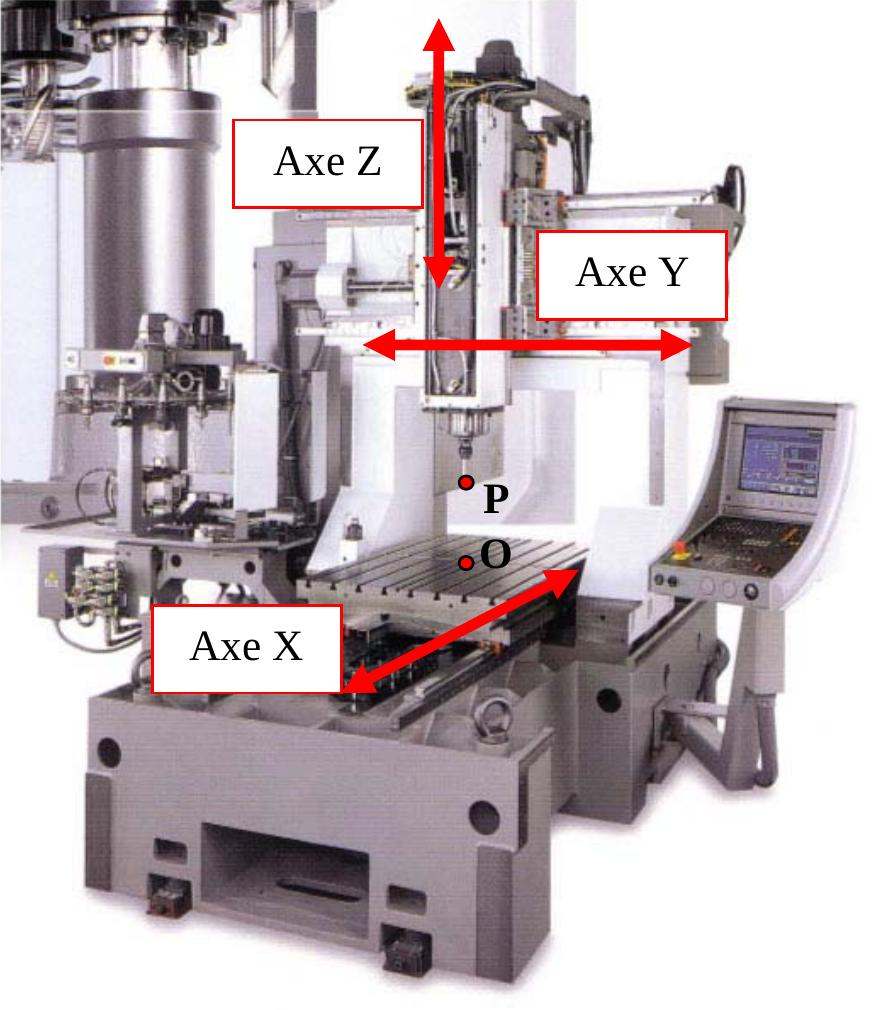
\includegraphics[width=\textwidth]{images/machineUGV}
% %\caption{Machine d'usinage grande vitesse}\label{machineUGV}
% \end{center}
% %\end{figure}
% \end{minipage}
% 
% On s'intéresse ici à la trajectoire du point $P$ dans son mouvement relatif au repère lié à la table de la
% machine, dont $O$ est l'origine. Les coordonnées du point $P$ dans l'espace sont notées $X$, $Y$ et $Z$.
% Une trajectoire 3D a été exécutée sur une machine de ce type et les coordonnées du point $P$ ont été
% enregistrées avec une période d'échantillonnage $T_e$, avec $T_e = 6\ \rm ms$. La trajectoire a été exécutée sur
% une machine d'Usinage à Grande Vitesse selon deux formats d'exécution (gérés par le Directeur de
% Commande Numérique de la machine)
% La vitesse d'avance du point $P$ (vitesse tangentielle à la trajectoire) a été programmée à $6\ \rm m/min$. Lors
% de l'usinage d'une pièce, il est préférable de conserver une vitesse d'avance constante afin de couper
% la matière dans de bonnes conditions. Malheureusement, les machines ayant des masses embarquées
% très importantes, les accélérations de chaque axe sont limitées pour éviter de détériorer la machine.
% Nous allons maintenant vérifier si la vitesse d'avance souhaitée est respectée le long de la trajectoire.
% Deux essais ont été conduits avec des méthodes de de génération de trajectoires différentes.
% 
% \subsection{Chargement de la trajectoire et visualisation}
% 
% Télécharger le dossier du TP (TP\_integ\_deriv\_num\_eleve) où se trouvent deux fichiers REC1.txt et REC2.txt, contenant les deux trajectoires d'outil.
% 
% \Question{Ouvrir le fichier REC1.txt dans un éditeur de texte, vérifier l'échantillonnage, et identifier le format des données. Écrire le programme python\footnote{Voir poly sur la lecture et l'écriture de fichiers ; il est plus simple de lire le fichier ligne à ligne par la commande readline().} permettant de charger les données dans des variables $T1$, $X1$, $Y1$ et $Z_1$.}
% 
% \Question{Tracer les trois composantes en fonction du temps et vérifier les ordres de grandeur du temps de déplacement de la machine et de l'amplitude des mouvements des axes.}
% 
% Le tracé d'une courbe 3D n'est pas très induitif sous python. Ouvrir le fichier courbe3D.py qui donne un exemple de tracé d'une courbe 3D.
% 
% \Question{Reprendre les commandes de l'exemple pour tracer la trajectoire à partir des coordonnées provenant du fichier.}
% 
% \Question{Charger de même la trajectoire enregistrée dans le fichier REC2.txt et vérifier qu'il s'agit bien de la même trajectoire. Comparer les durées des mouvements et les déplacements des axes $X$, $Y$ et $Z$ pour les deux trajectoires.}
% 
% \subsection{Validation de la vitesse d'avance}
% 
% La vitesse d'avance est supposée constante et égale à 6 m/min. Pour vérifier cette valeur, nous souhaitons tracer l'évolution de la vitesse au cours du temps.
% 
% Pour cela, nous calculerons d'abord l'abscisse curviligne puis, en dérivant, la vitesse de l'outil.
% 
% L'abscisse curviligne au point $P$ est la distance parcourue par l'outil depuis le début de la trajectoire. L'abscisse curviligne au départ est donc nulle et vaut la longueur totale de la trajectoire à la fin de son exécution.
% 
% 
% \Question{Écrire le programme permettant de calculer une liste contenant l'abscisse curviligne de chaque point de la trajectoire.}
% 
% \Question{Par une dérivation numérique à 1 pas (avant ou arrière), calculer la dérivée de l'abscisse curviligne, c'est-à-dire la vitesse de l'outil. Comparer les vitesses pour les deux trajectoires aux $6\ \rm m/min$ demandés.}


\section{Mesure d'une position par un capteur accélérométrique}

Un capteur accélérométrique permet de mesurer une accélération. Il est généralement constitué d'une masselotte fixée au boitier de la pièce en mouvement par un ressort. L'élongation du ressort permet de déterminer l'accélération du boitier par rapport à un référentiel galiléen. Ces composants ont été largement miniaturisés durant les 10 dernières années pour s'intégrer aux téléphones portables, tablettes, manettes de jeux et autres objets électroniques ayant besoin de mesurer un mouvement.

\begin{figure}[!h]
\begin{minipage}{0.45\linewidth}
\begin{center}
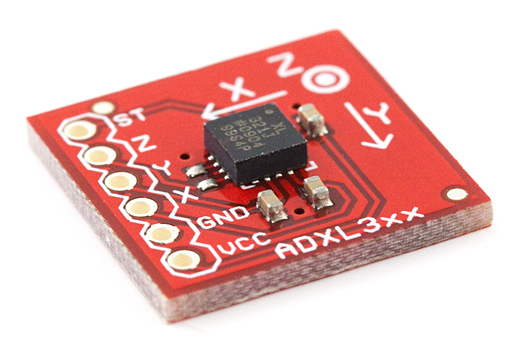
\includegraphics[width=.6\textwidth]{images/accelero}
\caption{Accéléromètre miniature}\label{accelero}
\end{center}
\end{minipage}\hfill
\begin{minipage}{0.45\linewidth}
\begin{center}
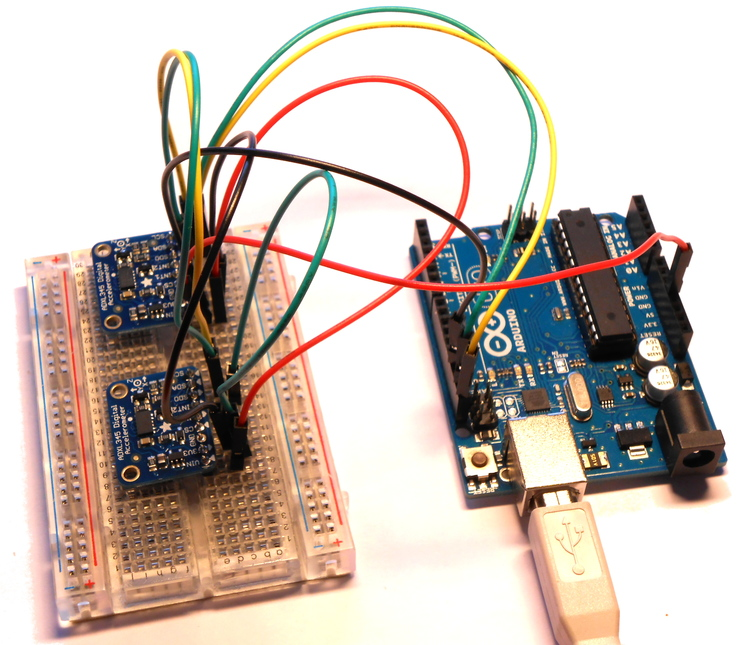
\includegraphics[width=.7\textwidth]{images/photo_arduino_accelero_petit}
\caption{Montage de l'accéléromètre sur l'arduino pour la mesure}\label{photo_arduino_accelero_petit}
\end{center}
\end{minipage}
\end{figure}

Ce problème vise à tester les possibilités de mesure de ces composants : peut-on, à partir de la mesure de l'accélération, remonter facilement à la vitesse, voire à la trajectoire du boitier dans lequel est monté le capteur ?

Pour les besoins du test, un capteur accélérométrique à été branché sur un arduino chargé de récupérer les mesures par un bus I2C et de retransmettre ces mesures à l'ordinateur par un protocole série. Les données envoyées par l'arduino sont pour chaque ligne : l'intervalle de temps écoulé depuis la précédente mesure (en micro-secondes) et les accélérations mesurées suivant $X$, $Y$ et $Z$.

Au début de la mesure, le capteur est à l'arrêt, à plat, durant quelques secondes puis il est déplacé en translation pour décrire un carré horizontal de coté environ égal à $0.5 \ \rm m$. Le fichier de point est fourni dans le dossier du TP : mesure\_accelero.txt.

\subsection{Importation des mesures et visualisation}

\Question{Ouvrir le fichier de mesure et identifier le format des données. L'échantillonnage est-il constant comme dans le cas de la trajectoire d'usinage ? Écrire le programme permettant de charger les données dans les variables $DT$, $AX$, $AY$ et $AZ$.}

Les pas de temps $DT$ sont donnés en micro-secondes mais ne permettent pas en l'état de tracer l'évolution des courbes d'accélération en fonction du temps. Par ailleurs, les accélérations sont données en incréments et doivent être étalonnées, sachant que $10\ \rm ms^{-2}$ correspond à 255 incréments.

\Question{Écrire le programme permettant de calculer un vecteur des temps $T$ qui permettra de tracer les courbes en fonction du temps (en secondes). Étalonner les courbes de façon à exprimer les données en $\rm ms^{-2}$.}

\Question{Tracer les trois courbes d'accélération. Que constatez vous en début d'essai lorsque le capteur est immobile ? Pouvez-vous interpréter les valeurs d'accélération obtenues ?}



\subsection{Intégration de l'accélération et traitement des mesures}

Pour obtenir la vitesse de déplacement, il faut intégrer l'accélération.

\Question{Proposer un programme permettant de calculer les composantes de vitesses $VX$, $VY$ et $VZ$. Tracer l'évolution des composantes de vitesses : que constatez vous ?}

Pour un résultat exploitable, une première précaution consiste à régler l'offset en début de mesure.

\Question{Calculer les moyennes des mesures d'accélération dans les trois directions durant le temps de repos et retrancher cette valeur aux courbes de façon à assurer une accélération nulle en moyenne en début d'essai. Refaire le calcul des vitesses et interpréter les courbes obtenues.}


\subsection{Double intégration et tracé de trajectoires}

\Question{Intégrer à nouveau les composantes de vitesse de façon à obtenir les composantes de position du capteur. Traçer les courbes et interpréter le résultat.}

\Question{Tracer la trajectoire du capteur calculée dans le plan $(\vec x,\vec y)$ et conclure sur les possibilités de mesure de position à l'aide d'un capteur accélérométrique.}




\section{Génération de trajectoire pour une imprimante 3D}

Une imprimante 3D est un appareil permettant de fabriquer un objet volumique (généralement en plastique) par ajout de matière. Les imprimantes grand publique sont constituées d'une tête chauffante faisant fondre un fil de plastique pour le déposer sur la zone à imprimer. La tête est montées sur 3 axes de translation de façon à déposer le fil fondu et progressivement former la géométrie de la pièce à fabriquer.

\begin{figure}[!h]
\begin{minipage}{0.55\linewidth}
\begin{center}
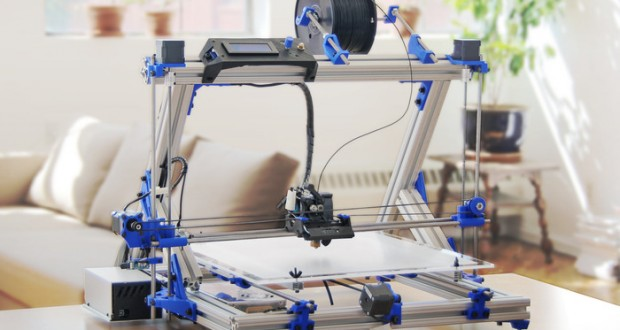
\includegraphics[width=.9\textwidth]{images/imprimante3D}
\caption{Imprimante 3D cartésienne grand public}\label{imprimante3D}
\end{center}
\end{minipage}\hfill
\begin{minipage}{0.35\linewidth}
\begin{center}
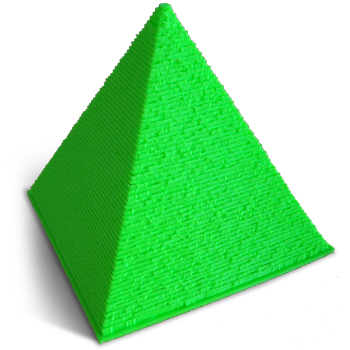
\includegraphics[width=.7\textwidth]{images/pyramide}
\caption{Pyramide imprimée sur une imprimante 3D}\label{pyramide}
\end{center}
\end{minipage}
\end{figure}

La tête est régulée en température de façon à faire fondre à la bonne température le fil. Néanmoins, l'asservissement étant lent, le fil doit sortir à une vitesse constante pour maintenir les bons réglages. Cette contrainte impose à la tête de parcourir une trajectoire à vitesse constante elle aussi.

Nous cherchons dans se problème à générer la trajectoire de consigne pour la tête d'impression, de façon à créer une pyramide miniature.

\subsection{Trajectoire pour former une pyramide}

La génération de la trajectoire brute (sans tenir compte de la vitesse de déplacement) nécessitant un peu de temps, le programme vous est donné dans le fichier pyramide.py.

\Question{Ouvrir le fichier et exécuter les commandes de façon à observer la trajectoire brute calculée.}


\subsection{Génération de la trajectoire machine}
Cette trajectoire brute est constituée de segments plus ou moins long, mais ne présente aucun échantillonnage temporel : chaque segment visible est uniquement constitué de deux points extrémité.

Pour obtenir une trajectoire machine, il faut échantillonner la courbe en pas de temps réguliers de $10\ \rm ms$ en assurant une vitesse constante de $V_0=1\ \rm mm/s$.

\Question{Créer une liste de temps pour la trajectoire brute, en considérant que chaque segment est parcouru à la vitesse $V_0$.}

\Question{Créer une liste de temps pour la trajectoire machine (en secondes).}

\Question{Calculer par interpolation les coordonnées $(x,y,z)$ pour chaque pas de temps machine puis tracer la trajectoire machine de façon à s'assurer qu'elle est bien identique à la trajectoire brute.}

\Question{Calculer la vitesse d'avance obtenue par la trajectoire machine et vérifier qu'elle est bien constante et égale à $V_0$.}


\end{document}






























\begin{minipage}[c]{.79\linewidth}
\section{Pourquoi utiliser des fichiers ?}

L'ordinateur sert à traiter de l'information qui peut entrer et sortir via
différentes interfaces :
\begin{itemize}
\item Le clavier, la souris et l'écran, pour l'interface utilisateur du programme ou le shell,
\item Les fichiers, pour les supports mémoire,
\item Les interfaces de communication (réseau, port USB, port série, etc).
\end{itemize}

Le clavier et la souris ne permettent pas d'entrer une grosse masse d'information.
De même l'écran montre une petite partie de l'information.
En revanche les fichiers permettent de décupler les possibilités de traitement d'information des programmes. Un roman de 200 pages contient environ 500 000 caractères, et donc tient en un fichier de 500 ko environ. 

Le réseau permet d'échanger des informations sous deux formes :
\begin{itemize}
\item Sous forme de fichiers échangés, qui sont ensuite stockés sur le disque dur.
\item Sous forme de flux de données. Ces données sont traitées par les cartes interfaces et mises à disposition des programmes par l'OS sous une forme proche des fichiers.
\end{itemize}
Il est donc intéressant de savoir lire et écrire sur les fichiers. 


\end{minipage} \hfill
\begin{minipage}[c]{.19\linewidth}
\begin{center}
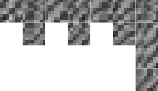
\includegraphics[width=.9\textwidth]{images/image1.png}
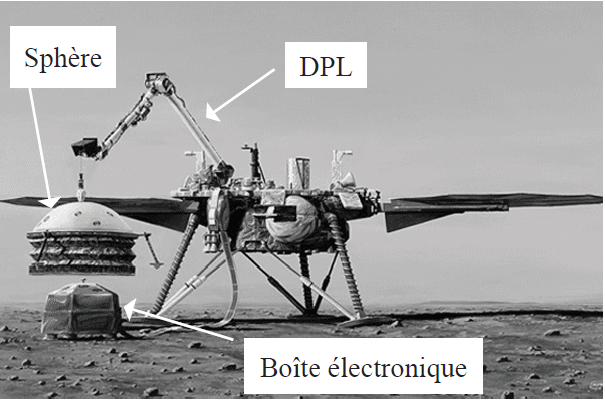
\includegraphics[width=.9\textwidth]{images/image2.png}
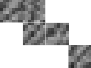
\includegraphics[width=.9\textwidth]{images/image3.png}
\end{center}




\end{minipage}






\subsection{Deux familles de fichiers}

Les fichiers sont tous écrits en binaire. Il est néanmoins possible de les séparer en deux familles :
\begin{minipage}[c]{.59\linewidth}



\begin{itemize}
\item Les fichiers binaires qui nécessitent de connaître le format binaire d'écriture des données pour être lus,
\item Les fichiers texte qui contiennent des caractères uniquement, et qui peuvent s'ouvrir sur un éditeur de texte.
\end{itemize}

\begin{exemple}

Les fichiers binaires :

\begin{itemize}
\item Images et documents (bmp, png, jpg, pdf, doc, etc)
\item Son et vidéo (wav, mp3, mp4, etc)
\item Exécutables (.exe)
\item Archives compressées (zip, 7z, gz)
\end{itemize}

Les fichiers texte :

\begin{itemize}
\item Pages Web (html, css, etc)
\item Fichier journal (log), Script shell (bat)
\item Images vectorielles (svg)
\item Programmes Python ou Scilab (py, sce)
\item Les fichiers de données texte (txt, data, etc)
\item Les fichiers texte formatés (xml)
\end{itemize}

Les fichiers texte compressés :
\begin{itemize}
\item Les fichiers bureautique (odt, ods, docx, xlsx)
\end{itemize}
\end{exemple}

\end{minipage} \hfill
\begin{minipage}[c]{.39\linewidth}
\begin{center}
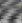
\includegraphics[width=.99\textwidth]{images/image4.png}
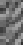
\includegraphics[width=.99\textwidth]{images/image5.png}
\end{center}
\end{minipage}





\subsection{Avantages et inconvénients}
\begin{center}
\begin{tabular}{|p{2.5cm}|p{6.5cm}|p{8cm}|}
\hline
 & Les fichiers binaires& Les fichiers texte\\
 \hline
Avantages &  Moins volumineux & Interprétables par l'homme\\

		  & Indépendants des standarts d'encodage des caractères dans les OS &Permettent des d'échanges plus simples entre logiciels\\
		  & & Ne nécessitent généralement pas de bibliothèques\\
\hline
Inconvénients & Moins faciles à lire & Plus volumineux\\

			& Nécessitent des bibliothèques pour les ouvrir &Dépendants du format d'encodage des caractères\\
			\hline
\end{tabular}
\end{center}

\vspace{-1cm}


\section{Fichiers binaires}

\vspace{-1cm}
\begin{figure}[H]
\begin{minipage}[c]{.53\linewidth}



\subsection{Analyse d'un fichier binaire : BMP}

On peut ouvrir un fichier binaire avec un éditeur héxadécimal.

Les deux premiers caractères de cette exemple "42" représentent en hexadécimal le codage sur les 8 bits correspondants (celui-ci apparait en bas de la fenêtre quand on se place sur le "42").

Un fichier BMP est un format très simple pour mémoriser les images:
\begin{itemize}
\item Signature (BM, BA, CI, …)
\item Taille du fichier (4o)
\item Champ réservé (4o)
\item Offset de début données (4o)
\item Taille de l'entête (4o)
\item Largeur de l'image (4o)
\item Hauteur de l'image (4o)
\item Nombre de plans (2o)
\item Profondeur : 1 à 32 (2o)
\item Type compression (4o)
\item Etc...
\end{itemize}


Les couleurs commencent à l'octet 122=0x7A (octet en jaune) :
\begin{itemize}
\item Blanc (ff ff ff),
\item Blanc (ff ff ff),
\item Blanc (ff ff ff),
\item Blanc (ff ff ff),
\item Gris clair (e9 ec ef),
\item Gris (ce cc c4),
\item Gris foncé (a0 97 7c)...
\end{itemize}
\begin{center}
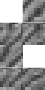
\includegraphics[width=.5\textwidth]{images/image8.png}
\end{center}
\end{minipage} \hfill
\begin{minipage}[c]{.45\linewidth}
\begin{center}
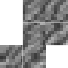
\includegraphics[width=.5\textwidth]{images/image6.png}
\end{center}
\begin{center}
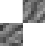
\includegraphics[width=.99\textwidth]{images/image12.png}
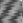
\includegraphics[width=.99\textwidth]{images/image13.png}
\caption{Ouverture d'un fichier binaire avec un éditeur hexadécimal}
\end{center}
\end{minipage}
\end{figure}







\subsection{Ouvrir des fichiers binaires}
Les formats étant généralement assez complexes et variés, les fichiers binaires sont ouverts via des \textbf{librairies}. Ces librairies proposent des commandes toutes prêtes. Par exemple pour les images :
\begin{itemize}
\item Python : Librairie PIL (Python Imaging Library).
\item Scilab inclut des commandes pour les images
\end{itemize}

On code très rarement les commandes permettant d'ouvrir les fichiers binaires.
Pour lire tout de même un fichier binaire on utilise la fonction open, disponible sans avoir besoin de rien importer. Elle prend en paramètre :
\begin{itemize}
\item le chemin (absolu ou relatif) menant au fichier à ouvrir ;
\item le mode d'ouverture.
\end{itemize}

Le mode est donné sous la forme d'une chaîne de caractères. Voici les principaux modes :
\begin{itemize}
\item 'r' : ouverture en lecture (Read).
\item 'w' : ouverture en écriture (Write). Le contenu du fichier est écrasé. Si le fichier n'existe pas, il est créé.
\item 'a' : ouverture en écriture en mode ajout (Append). On écrit à la fin du fichier sans écraser l'ancien contenu du fichier. Si le fichier n'existe pas, il est créé.
\end{itemize}

On peut ajouter à tous ces modes le signe b pour ouvrir le fichier en mode binaire.

%La fonction open crée un objet de la classe TextIoWrapper. Par la suite, nous allons utiliser des méthodes de cette classe pour interagir avec le fichier.

\begin{minipage}[c]{.49\linewidth}

\begin{py}
\begin{python}[H]
# Lecture d'un fichier binaire
f = open("tongue.bmp", "rb")

while True:
	bytes = f.read(1) # lecture d'un octet
	if bytes == "":
	    break;
	# Affichage de l'octet lu en hexadécimal :
	print "%02X " % ord(bytes[0]),

f.close()
\end{python}
\end{py}



\end{minipage} \hfill
\begin{minipage}[c]{.49\linewidth}
3 étapes:
\begin{itemize}
\item Ouverture du fichier “tongue.bmp”, en lecture mode binaire (“rb”).
\item Boucle sur chaque octet pour lire et afficher. La méthode read renvoie le contenu du fichier, que l'on capture dans bytes.
\item Fermeture du fichier: n'oubliez pas de fermer un fichier après l'avoir ouvert. Si d'autres applications, ou d'autres morceaux de votre propre code, souhaitent accéder à ce fichier, ils ne pourront pas car le fichier sera déjà ouvert. C'est surtout vrai en écriture, mais prenez de bonnes habitudes. La méthode à utiliser est close.
\end{itemize} 
\end{minipage}


\subsection{Écrire dans des fichiers en binaire}


\begin{minipage}[c]{.39\linewidth}

\begin{py}
\begin{python}[H]
# Écriture d'un fichier binaire
f=open("TP/monFichier.bin","wb")
f.write("Du texte")
f.write(int8(83))
f.write(int8(76))
f.write(float32(2.3))
f.close()
\end{python}
\end{py}

\end{minipage} \hfill
\begin{minipage}[c]{.59\linewidth}
3 étapes:
\begin{itemize}
\item Il faut ouvrir le fichier avant tout. Ouverture du fichier “monFichier.bin”, en écriture mode binaire (“wb”).
\item Écriture d'octets (caractères, nombres entiers ou flottants): On utilise la méthode write. Deux modes sont possibles: le mode w ou le mode a. Le premier écrase le contenu éventuel du fichier, alors que le second ajoute ce que l'on écrit à la fin du fichier. Ces deux modes créent le fichier s'il n'existe pas.
\item Fermeture du fichier. 
\end{itemize}
\end{minipage}





\section{Fichiers texte}


Un fichier texte brut ou fichier texte simple est un fichier dont le contenu représente uniquement une suite de caractères.
Bien qu'on l'oppose ici aux fichiers binaires il est lui aussi codé en binaire sur l'ordinateur. Cependant ce codage est basé sur une norme connue de tous les éditeurs de texte afin de traduire le fichier en une suite de caractères "imprimables".
Les caractères considérés sont généralement les caractères imprimables, d'espaces et de retours à la ligne. La notion de fichier texte est subjective et dépend notamment des systèmes de codage de caractère considérés. Ainsi si l'encodage est inconnu, un texte brut quelconque est inexploitable.

 





\begin{figure}[H]
\begin{minipage}[c]{.49\linewidth}
Il existe de nombreux standards de codage, dont l'American Standard Code for Information Interchange   ASCII. Cette norme ancienne créée pour gérer des caractères latins non accentués (nécessaire pour écrire en anglais) est à la base de nombreux codages de caractères.
\newline\newline L'ASCII permet de coder 128 caractères numérotés de 0 à 127 et peut donc être codé sur 7 bits. Cependant, les ordinateurs travaillent la plupart du temps en multiple de 8 bits, le huitième bit est mis à 0. On a donc un octet par caractère.
\newline\newline L'absence d'accents rend cette norme insuffisante à elle seule,
ce qui rend nécessaire l'utilisation d'autres encodages: UTF-8 par exemple (UCS transformation format 8 bits) dans lequel chaque caractère est représenté par un index et son codage binaire donné par une table. Les 128 premiers caractères ont un codage identique en ASCII et UTF8 (Par exemple "A" a pour code ASCII 65 et se code en UTF-8 par l'octet 65.) puis d'autres caractères sont ajoutés.


\end{minipage} \hfill
\begin{minipage}[c]{.49\linewidth}
\begin{center}
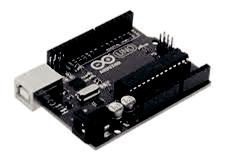
\includegraphics[width=.99\textwidth]{images/image14.png}
\caption{Table des caractères ASCII}
\end{center}
\end{minipage}
\end{figure}

\subsection{Lecture d'un fichier sous Python}


\begin{minipage}[c]{.63\linewidth}


Les fichiers texte sont écrits (en binaire) de façon à respecter un des codes standards de caractères (utf8, iso-8859, ASCII...).
Ils peuvent s'ouvrir sur un éditeur de texte, ce qui permet de lire ou modifier le contenu beaucoup plus facilement qu'en binaire.

\textsc{Exemple} : fichier de mesure sur l'axe Emericc: 
$Mesure\_axe\_Emericc.txt$

\textbf{\textsc{Objectif} : Lire les données (paramètres et mesures) et tracer les courbes.}

\begin{itemize}
\item 12 lignes de paramètres
\item 100 lignes de données
\item 9 lignes de paramètres
\end{itemize}

Lecture des noms:
\begin{py}
\begin{python}[H]
# Lecture d'un fichier texte ligne à ligne
# Ouverture fichier
f=open("TP_Fichiers/Mesure_axe_Emericc.txt","r")
ligne = f.readline()                  # lecture d'une ligne
# Affichage pour vérification
print "%s" % ligne
ligne=ligne.rstrip("\n\r")            # suppression retour chariot
noms_grandeurs=ligne.split("\t")      # découpage aux tabulations
noms_grandeurs=noms_grandeurs[1:3]    # suppression de "noms"

\end{python}
\end{py}
\end{minipage} \hfill
\begin{minipage}[c]{.36\linewidth}

\begin{center}
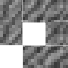
\includegraphics[width=.99\textwidth]{images/image11.png}
\end{center}

\end{minipage}


Lecture du nombre de points:
\begin{py}
\begin{python}[H]
for i in range(10):
    ligne = f.readline()  # saut de 10 lignes

ligne = f.readline()                  # lecture d'une ligne 
print "%s" % ligne                    # affichage pour vérification
ligne=ligne.rstrip("\n\r")            # suppression retour chariot
ligne_nbpoints=ligne.split("\t")      # découpage aux tabulations
nb_points=int(ligne_nbpoints[1])      # convertion en entier
\end{python}
\end{py}

\newpage
Lecture des données:
\begin{py}
\begin{python}[H]

numero=[] ; position=[] ; consigne=[] # initialisation tableaux

for i in range(nb_points):
    ligne = f.readline()              # lecture d'une ligne 
    ligne=ligne.rstrip("\n\r")        # suppression retour chariot
    ligne=ligne.replace(",",".")      # changement , en .
    ligne_data=ligne.split("\t")      # découpage aux tabulations
    numero.append(int(ligne_data[0]))
    position.append(float(ligne_data[1]))    # Ajout aux tableaux
    consigne.append(float(ligne_data[2]))
\end{python}
\end{py}



\begin{minipage}[c]{.49\linewidth}
Fermeture du fichier et Tracé de la courbe
\begin{py}
\begin{python}[H]

f.close()        # Fermeture fichier

plot(position)   # Tracé de la courbe de position
\end{python}
\end{py}
\end{minipage} \hfill
\begin{minipage}[c]{.49\linewidth}
\begin{center}
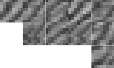
\includegraphics[width=.99\textwidth]{images/image9.png}
\end{center}
\end{minipage}



\subsection{Lecture d'un fichier sous Scilab}

De la même façon que Python, Scilab permet de lire des fichiers. La syntaxe est proche :

\begin{sci}
\begin{scilab}[H]
// Ouverture du fichier et lecture ligne à ligne
fic=mopen("Mesure_axe_Emericc.txt","r");
ligne=mgetl(fic,1)
// Découpage à   la tabulation = caractère ascii 9
noms_grandeurs=strsplit(ligne,ascii(9))
noms_grandeurs=noms_grandeurs(2:3)
for i=1:10
    ligne = mgetl(fic,1);
end

ligne = mgetl(fic,1)
ligne_nbpoints=strsplit(ligne,ascii(9))
nb_points=int(ligne_nbpoints(2))
nb_points=msscanf(ligne_nbpoints(2),"%i")
\end{scilab}
\end{sci}


Lecture des données et affichage de la courbe.

\begin{sci}
\begin{scilab}[H]
numero=[];position=[];consigne=[];
for i=1:nb_points
    ligne = mgetl(fic,1);
    ligne = strsubst(ligne,",",".");
    [n,numero(i),position(i),consigne(i)]=msscanf(ligne,"%d\t%f\t%f");
end
mclose(fic);                    // Fermeture du fichier
plot(position)
\end{scilab}
\end{sci}




\begin{minipage}[c]{.69\linewidth}

\subsection{Cas des données formatées}
Le tableau de données est “formaté”, c'est-à-dire qu'il présente une structure identique à chaque ligne.

Python possède des outils de lecture automatique de ce type de tableau : numpy.loadtxt()

\begin{py}
\begin{python}[H]
a=loadtxt("Fichier.txt",
		dtype={
			'names': ('numero', 'position', 'consigne'),
			'formats': ('i2', 'f4', 'f4')},
		delimiter='\t')
\end{python}
\end{py}

\end{minipage} \hfill
\begin{minipage}[c]{.29\linewidth}
\begin{tabular}{ccc}
\hline
Int	&float	&	float\\
\hline
0	&0,00		&8,00\\
1	&0,06	&	127,00\\
2&	0,23	&	127,00\\
3&	0,51	&	127,00\\
4&	0,88	&	119,00\\
5&	1,34	&	107,00\\
6&	1,91	&	92,00\\
7&	2,52	&	76,00\\
... &...  &...  \\
97&	4,94	&	1,00\\
98&	4,94	&	1,00\\
99&	4,94	&	1,00\\
\hline
\end{tabular}


\end{minipage}



Pour récupérer les données :
\begin{py}
\begin{python}[H]
a['numero']			#liste de valeurs de la colonne N
a['numero'][10]			#11ème élément
\end{python}
\end{py}


\begin{figure}[H]
\begin{minipage}[c]{.59\linewidth}

\begin{py}
\begin{python}[H]
a,b=loadtxt("Fichier.txt",
		usecols = (0,2),
		dtype={
			'names': ('numero', 'consigne'),
			'formats': ('i2', 'f4')},
		delimiter='\t',
		unpack=True)
\end{python}
\end{py}

\end{minipage} \hfill
\begin{minipage}[c]{.39\linewidth}
\begin{itemize}
\item usecols : colonnes à utiliser dans le fichier
\item dtype : type de données à lire
\item Names : nom
\item Format : entier sur 2o, flottant sur 4o, strings...
\item délimiter : séparateur des données
\item unpack : permet de séparer les colonnes → a,b=...
\end{itemize}
\end{minipage}
\end{figure}


\begin{figure}[H]
\begin{minipage}[c]{.49\linewidth}

\begin{py}
\begin{python}[H]
plot(a['numero'],a['position'],'b',
		a['numero'],a['consigne']/10,'r')
\end{python}
\end{py}

\end{minipage} \hfill
\begin{minipage}[c]{.49\linewidth}
\begin{center}
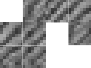
\includegraphics[width=.99\textwidth]{images/image10.png}
\end{center}
\end{minipage}
\end{figure}

\subsection{Lecture d'un fichier texte formaté sous Scilab}

\begin{figure}[H]
\begin{minipage}[c]{.49\linewidth}


De la même façon que Python, Scilab permet de lire des fichiers formatés.

La synthaxe est proche (en plus simple quand même...).

\end{minipage} \hfill
\begin{minipage}[c]{.49\linewidth}
\begin{sci}
\begin{scilab}[H]
// Lecture de données formatées
fic=mopen("Mesure_axe_Emericc_formate.txt","r");
T=mfscanf(-1,fic,'%d\t%f\t%f')  
plot(T(:,1),[T(:,2),T(:,3)/10])
mclose(fic);               // Fermeture du fichier
\end{scilab}
\end{sci}
\end{minipage}
\end{figure}




\subsection{Écriture d'un fichier texte sous python}
L'écriture d'un fichier texte est très simple sous python:
\begin{py}
\begin{python}[H]
# Écriture d'un fichier texte ligne à ligne
f=open("TP_Fichiers/monFichier.txt","w")  # Ouverture du fichier
f.write("La température est froide l'hiver.\n")
f.write("Il fait {:f} degrés.".format(10))
f.close()        # Fermeture du fichier
\end{python}
\end{py}

Et pour un fichier formaté :
\begin{py}
\begin{python}[H]
# Écriture d'un fichier formaté
f=open("TP/monFichier.txt","w")  # ouverture fichier
x=linspace(-20,20,100)
y=sin(x)/x
for i in range(0,len(x)):
    f.write("{:d} \t {:f} \t {:f}\n".format(i,x[i],y[i]))
f.close()        # Fermeture du fichier
\end{python}
\end{py}

\subsection{Écriture d'un fichier texte sous Scilab}
L'écriture d'un fichier texte, formaté ou pas, est très simple :
\begin{sci}
\begin{scilab}[H]
// Écriture de données formatées ou non...
fic=mopen("monFichier.txt","w");
mfprintf(fic,"Voici mon fichier de point\n")
mfprintf(fic,"Nombre de points : %d\n",100)
x=-20:40/99:20;
y=sin(x)./x;
mfprintf(fic,'%d\t%f\t%f\n',[1:100]',x',y')  
mclose(fic); // Fermeture du fichier
\end{scilab}
\end{sci}

\section{Enregistrer un objet dans un fichier: Module Pickle}

Dans Python comme dans beaucoup de langages de haut niveau, on peut enregistrer les objets dans un fichier. 
Lorsque l'objectif est de sauver des objets python pour les récupérer plus tard sous python, il est pratique d'utiliser Pickle.

Alors que les fonctions utilisées dans ce cours ne nécessitaient pas l'importation de bibliothèque, il faut penser ici à importer Pickle.

Soit v une variable quelconque,

\begin{minipage}[t]{.49\linewidth}

Sauvegarde :


\begin{py}
\begin{python}[H]
import pickle
fic=open("nao.pick","wb"")
pickle.dump(v,fic)
fic.close()
\end{python}
\end{py}

On utilise la méthode dump pour enregistrer l'objet.

Une fois ce code exécuté un fichier nao.pick aura été créé avec les données correspondantes à l'intérieur.

Pour stocker plusieurs variables, il suffit d'appeler plusieurs fois la fonction pickle.dump() pour chaque variable.

\end{minipage} \hfill
\begin{minipage}[t]{.49\linewidth}

Lecture :	

\begin{py}
\begin{python}[H]
import pickle
fic=open("nao.pick","rb"")
v=pickle.load(fic)
fic.close()
\end{python}
\end{py}



Pour recharger ces variables, il faut appeler autant de fois la fonction pickle.load(). Les variables sont restituées dans le même ordre.

\end{minipage}




\end{document}
